\subsection{Задача прогнозирования}
Результаты представляются графиком и таблицей для каждого пункта.
Координатой оси $X$ является идентификатор пользователя, координатой
оси $Y$ является значение оценки качества.
В качестве функции $\eit$ использовалась функция
NMAE \ref{nmae}.
Другие функции рассматривались так же, но между
функциями одного класса существует корреляция и приведение других графиков
оказывается избыточным.

На графиках представляются данные по двум методам тестирования. Для наглядности
результирующие данные были отсортированы по значениям оценки качества,
принадлежащим первому методу (в каждой паре точек, которые находятся на одной
вертикали, идентификаторы пользователей совпадают).

В таблицах представлены средние значения оценок точности по всем пользователям.

Для проведения тестов данного пункта исходные данные были
стандартно разбиты на тестовое и обучающее множество по следующему принципу:
разбиение проводилось случайно, в обучающее множество входит
80\% данных, в тестовое --- оставшиеся 20\%. В тестировании участвовало
подмножество $P^{\prime} \subset P, P^{\prime} = \{(u, i, \rho(u, i)):
\rho(u, i) = 1\}$.

\subsubsection{Влияние свойства транзитивности на СОМ при решении задачи
прогнозирования}
В данном пункте приведем и сравним результаты решения задачи $pred$, полученные:
\begin{enumerate}
	\item  в СОМ при следующих параметрах:
		\begin{itemize}
			\item
			стандартный алгоритма решения задачи
			$pred$ (\ref{alg:p-srs}), основанный на
			правиле вывода $\Pi_C$;
			\item
			пороговое значение $\Delta_u$ равно $0,9$;
			\item
		применяемая мера сходства --- коэффициент корреляции Пирсона
				(\ref{pearson}).
		\end{itemize}
	\item  в СОМ при следующих параметрах:
		\begin{itemize}
			\item
			стандартный алгоритма решения задачи
			$pred$ (\ref{alg:p-srs}), основанный на
			правиле вывода $\Pi_C$;
			\item
			пороговое значение $\Delta_u$ равно $0,49$;
			\item
		применяемая мера сходства --- коэффициент корреляции Пирсона
				(\ref{pearson}).
		\end{itemize}
\end{enumerate}

При $\Delta_u = 0,9$ вероятность того, что $(u \rt v) \wedge (v \rt z)
\Rightarrow (u \rt z)$, выше, чем при $\Delta_u = 0,49$.
На Рис. \ref{pic:predtrans} приведены результаты решений задачи $topN$ при
различных пороговых значениях. Черным цветом приведены результаты для
$\Delta_u = 0,9$, красным --- для $\Delta_u = 0,49$.
Видно, что при $\Delta_u = 0,9$ результаты решений эффективней, так
как большинство точек, соответствующих $\Delta_u = 0,9$ проходит ниже точек,
соответствующих $\Delta_u = 0,49$, что также подтверждается табличными данными,
представленными в таблице (\ref{tbl:predtrans}).

Некоторые результаты при $\Delta_u = 0,9$ хуже, чем при
$\Delta_u = 0,49$. Это происходит для тех пользователей,
для которых характерно свойство неоднородности.

\begin{figure}[H]
	\caption{Влияние свойства транзитивности на СОМ при решении задачи $pred$}
	\label{pic:predtrans}
	\begin{center}
		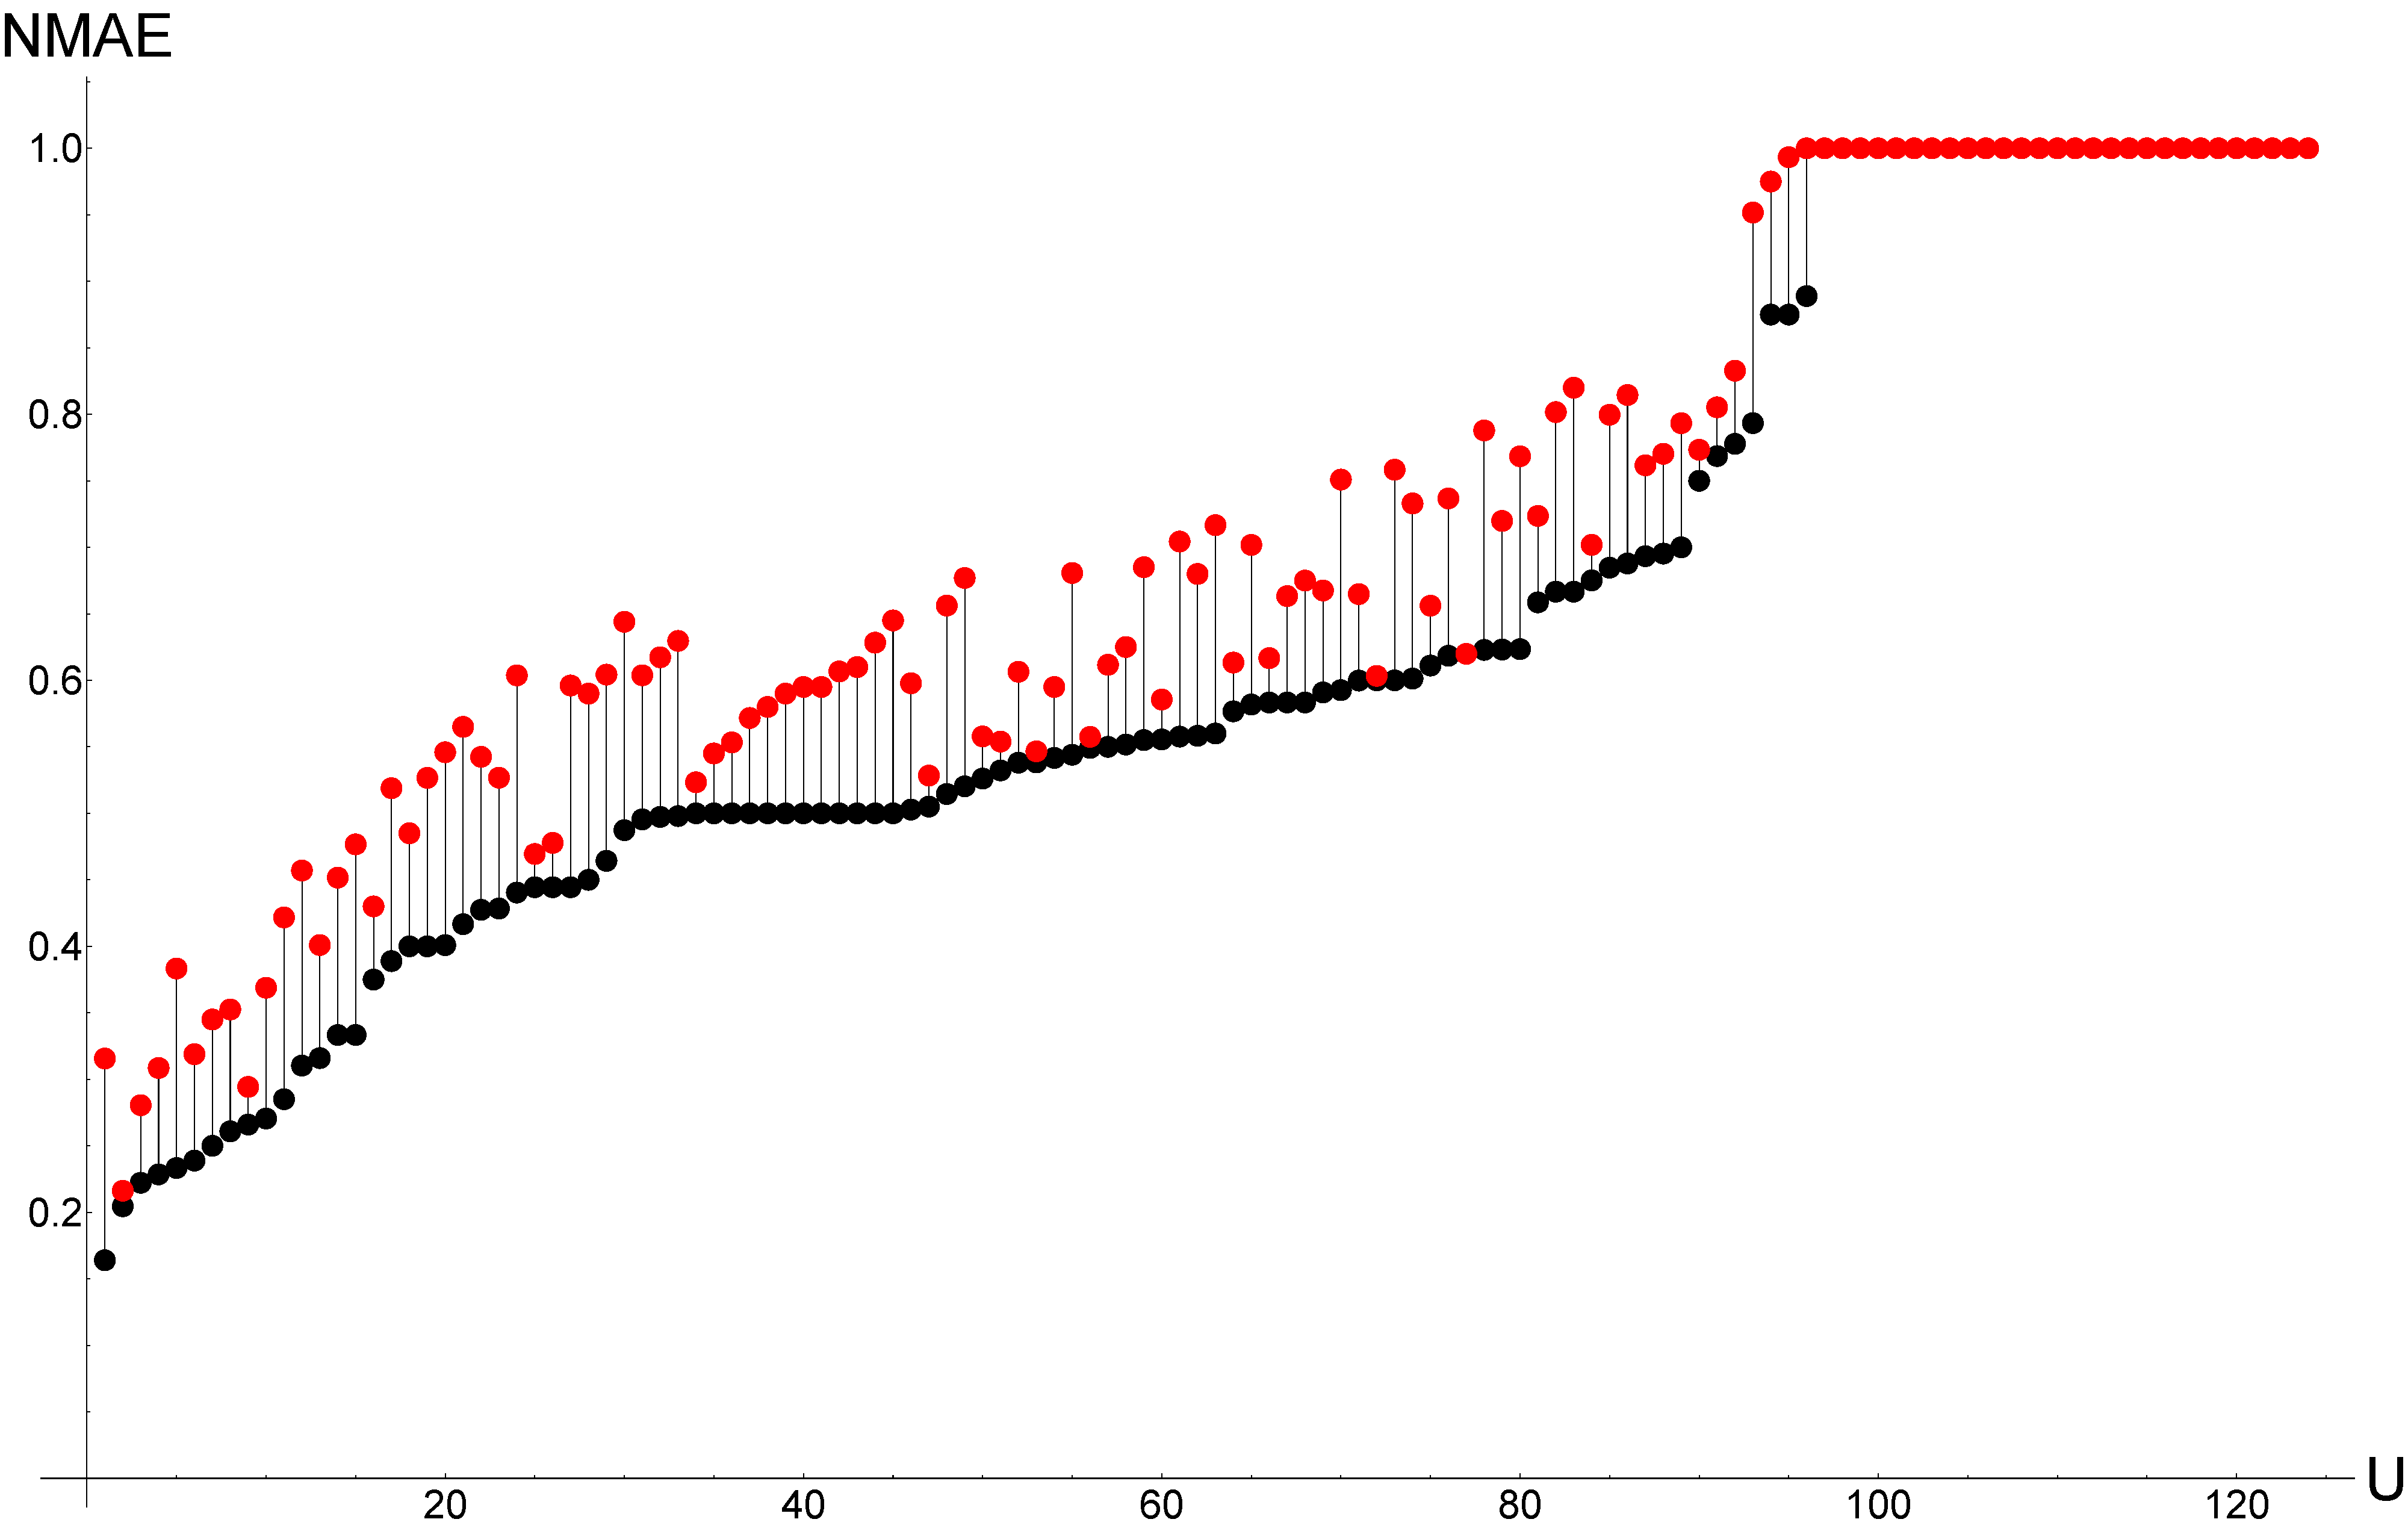
\includegraphics[width=7in,height=4in]{pics/results/ub_transitivity.pdf}
\end{center}
\end{figure}

\begin{table}[H]
	\caption{Влияние свойства транзитивности на СОМ при решении задачи $pred$}
  \label{tbl:predtrans}
  \begin{center}
	\begin{tabular}{|c|c|}
	  \hline
		Пороговое значение & NMAE \\ \hline
		0,9&0,495 \\ \hline
		0,49&0,601 \\ \hline
	\end{tabular}
  \end{center}
\end{table}

\subsubsection{Применение правила вывода СОМ в коллаборативной и нечеткой
моделях}
В данном пункте приведем и сравним результаты решения задачи $topN$, полученные:
\begin{enumerate}
	\item  в СОМ при следующих параметрах:
		\begin{itemize}
			\item
			стандартный алгоритма решения задачи
			$pred$ (\ref{alg:p-srs}), основанный на
			правиле вывода $\Pi_C$;
			\item
			пороговое значение $\Delta_u$ равно $0,9$;
			\item
		применяемая мера сходства --- коэффициент корреляции Пирсона
		\end{itemize}
	\item в нечеткой при следующих параметрах:
		\begin{itemize}
			\item
			стандартный алгоритма решения задачи
			$pred$ (\ref{alg:p-srs}), основанный на
			правиле вывода $\Pi_C$;
			\item
				применяемая мера сходства --- обобщенное расстояние Хэмминга
				(\ref{fuz:rhi})
		\end{itemize}
\end{enumerate}

На Рис. \ref{pic:predpio} приведены результаты решения
задачи $topN$ при применении $\Pi_C$ в СОМ и нечеткой модели.
Черным цветом обозначены результаты решения в нечеткой модели.
Видно, что в большинстве случаев нечеткая модель более эффективна
по критерию качества. В обратных ситуациях предпочтения пользователя
неоднородны.
%, и $\delta_c$ для таких пользователей определена так, что
%$|\rho(u, i) - \rh(u, i)| > \varepsilon_p$.

\begin{figure}[H]
	\caption{Качество решений при применении правила вывода $\Pi_{C}$ в нечеткой модели и СОМ}
	\label{pic:predpio}
	\begin{center}
		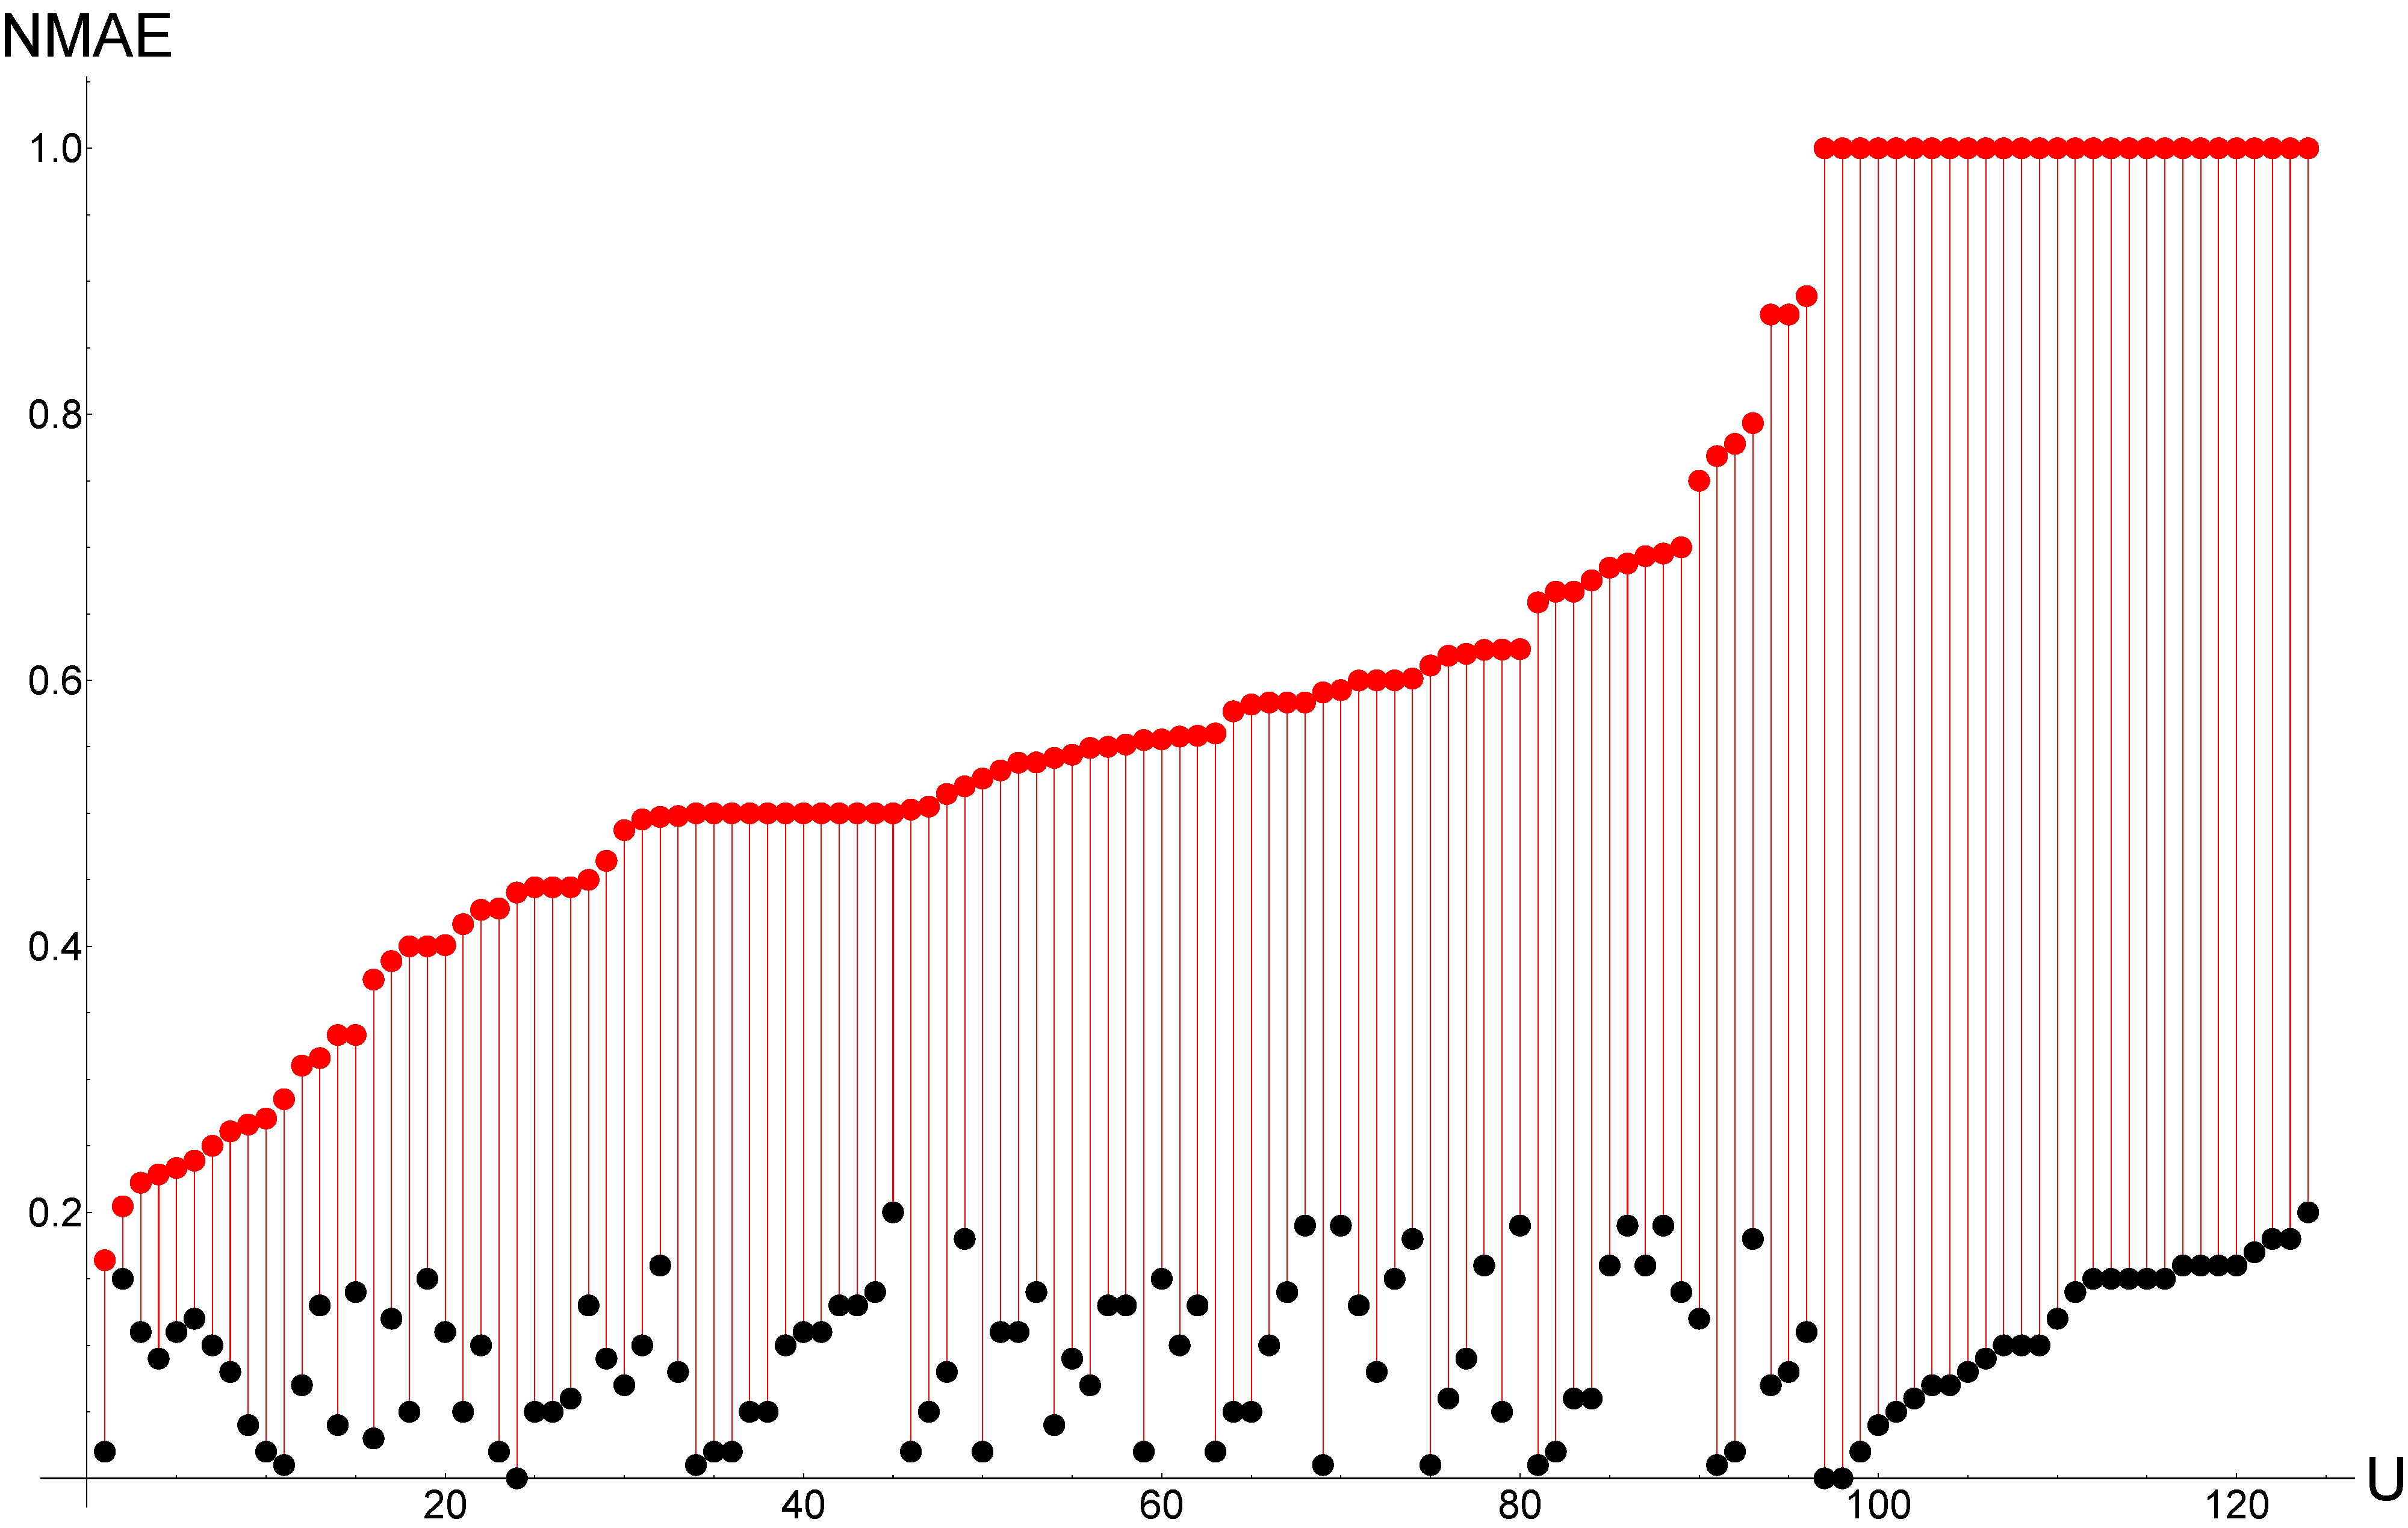
\includegraphics[width=7in,height=4in]{pics/results/ub_method_in_ub_and_fuzz_model.pdf}
\end{center}
\end{figure}

\begin{table}[H]
	\caption{Средняя точность решений при применении правила вывода $\Pi_{C}$ в нечеткой модели и СОМ}
  \label{tbl:predhamming}
  \begin{center}
	\begin{tabular}{|c|c|}
	  \hline
		Модель& Точность \\ \hline
		Нечеткая&0,001 \\ \hline
		COM&0,495\\ \hline
	\end{tabular}
  \end{center}
\end{table}

Практические результаты подтверждают вывод (\ref{trm:fuz-eff-com}) о том, что
применение $\Pi_C$ в нечеткой модели более эффективно по критерию качества,
чем применение того же правила в АКМ.

\subsubsection{Применение правила вывода нечеткой модели для решения задачи
$pred$}
В данном пункте приведем и сравним результаты решения задачи $pred$, полученные:
\begin{enumerate}
	\item в СОМ:
		\begin{itemize}
			\item
			стандартный алгоритма решения задачи
			$topN$ (\ref{alg:topn-solve-ors}), основанный на
			правиле вывода $\Pi_C$;
			\item
			пороговое значение $\Delta_u$ равно $0,9$;
			\item
		применяемая мера сходства --- косинус угла (\ref{sim-cos})
		между контентами, которые представляются в СОМ в виде векторов.
		\end{itemize}
	\item
		\begin{itemize}
			\item
			алгоритма решения задачи
			$pred$ (\ref{alg:fuz-p}), основанный на
			правиле вывода $\Pi_f$;
		\end{itemize}
\end{enumerate}


\begin{figure}[H]
	\caption{Качество решений задачи $pred$ при использовании $\Pi_C$ в СОМ и
	$\Pi_f$ в нечеткой модели}
	\label{pic:predpio_pif}
	\begin{center}
		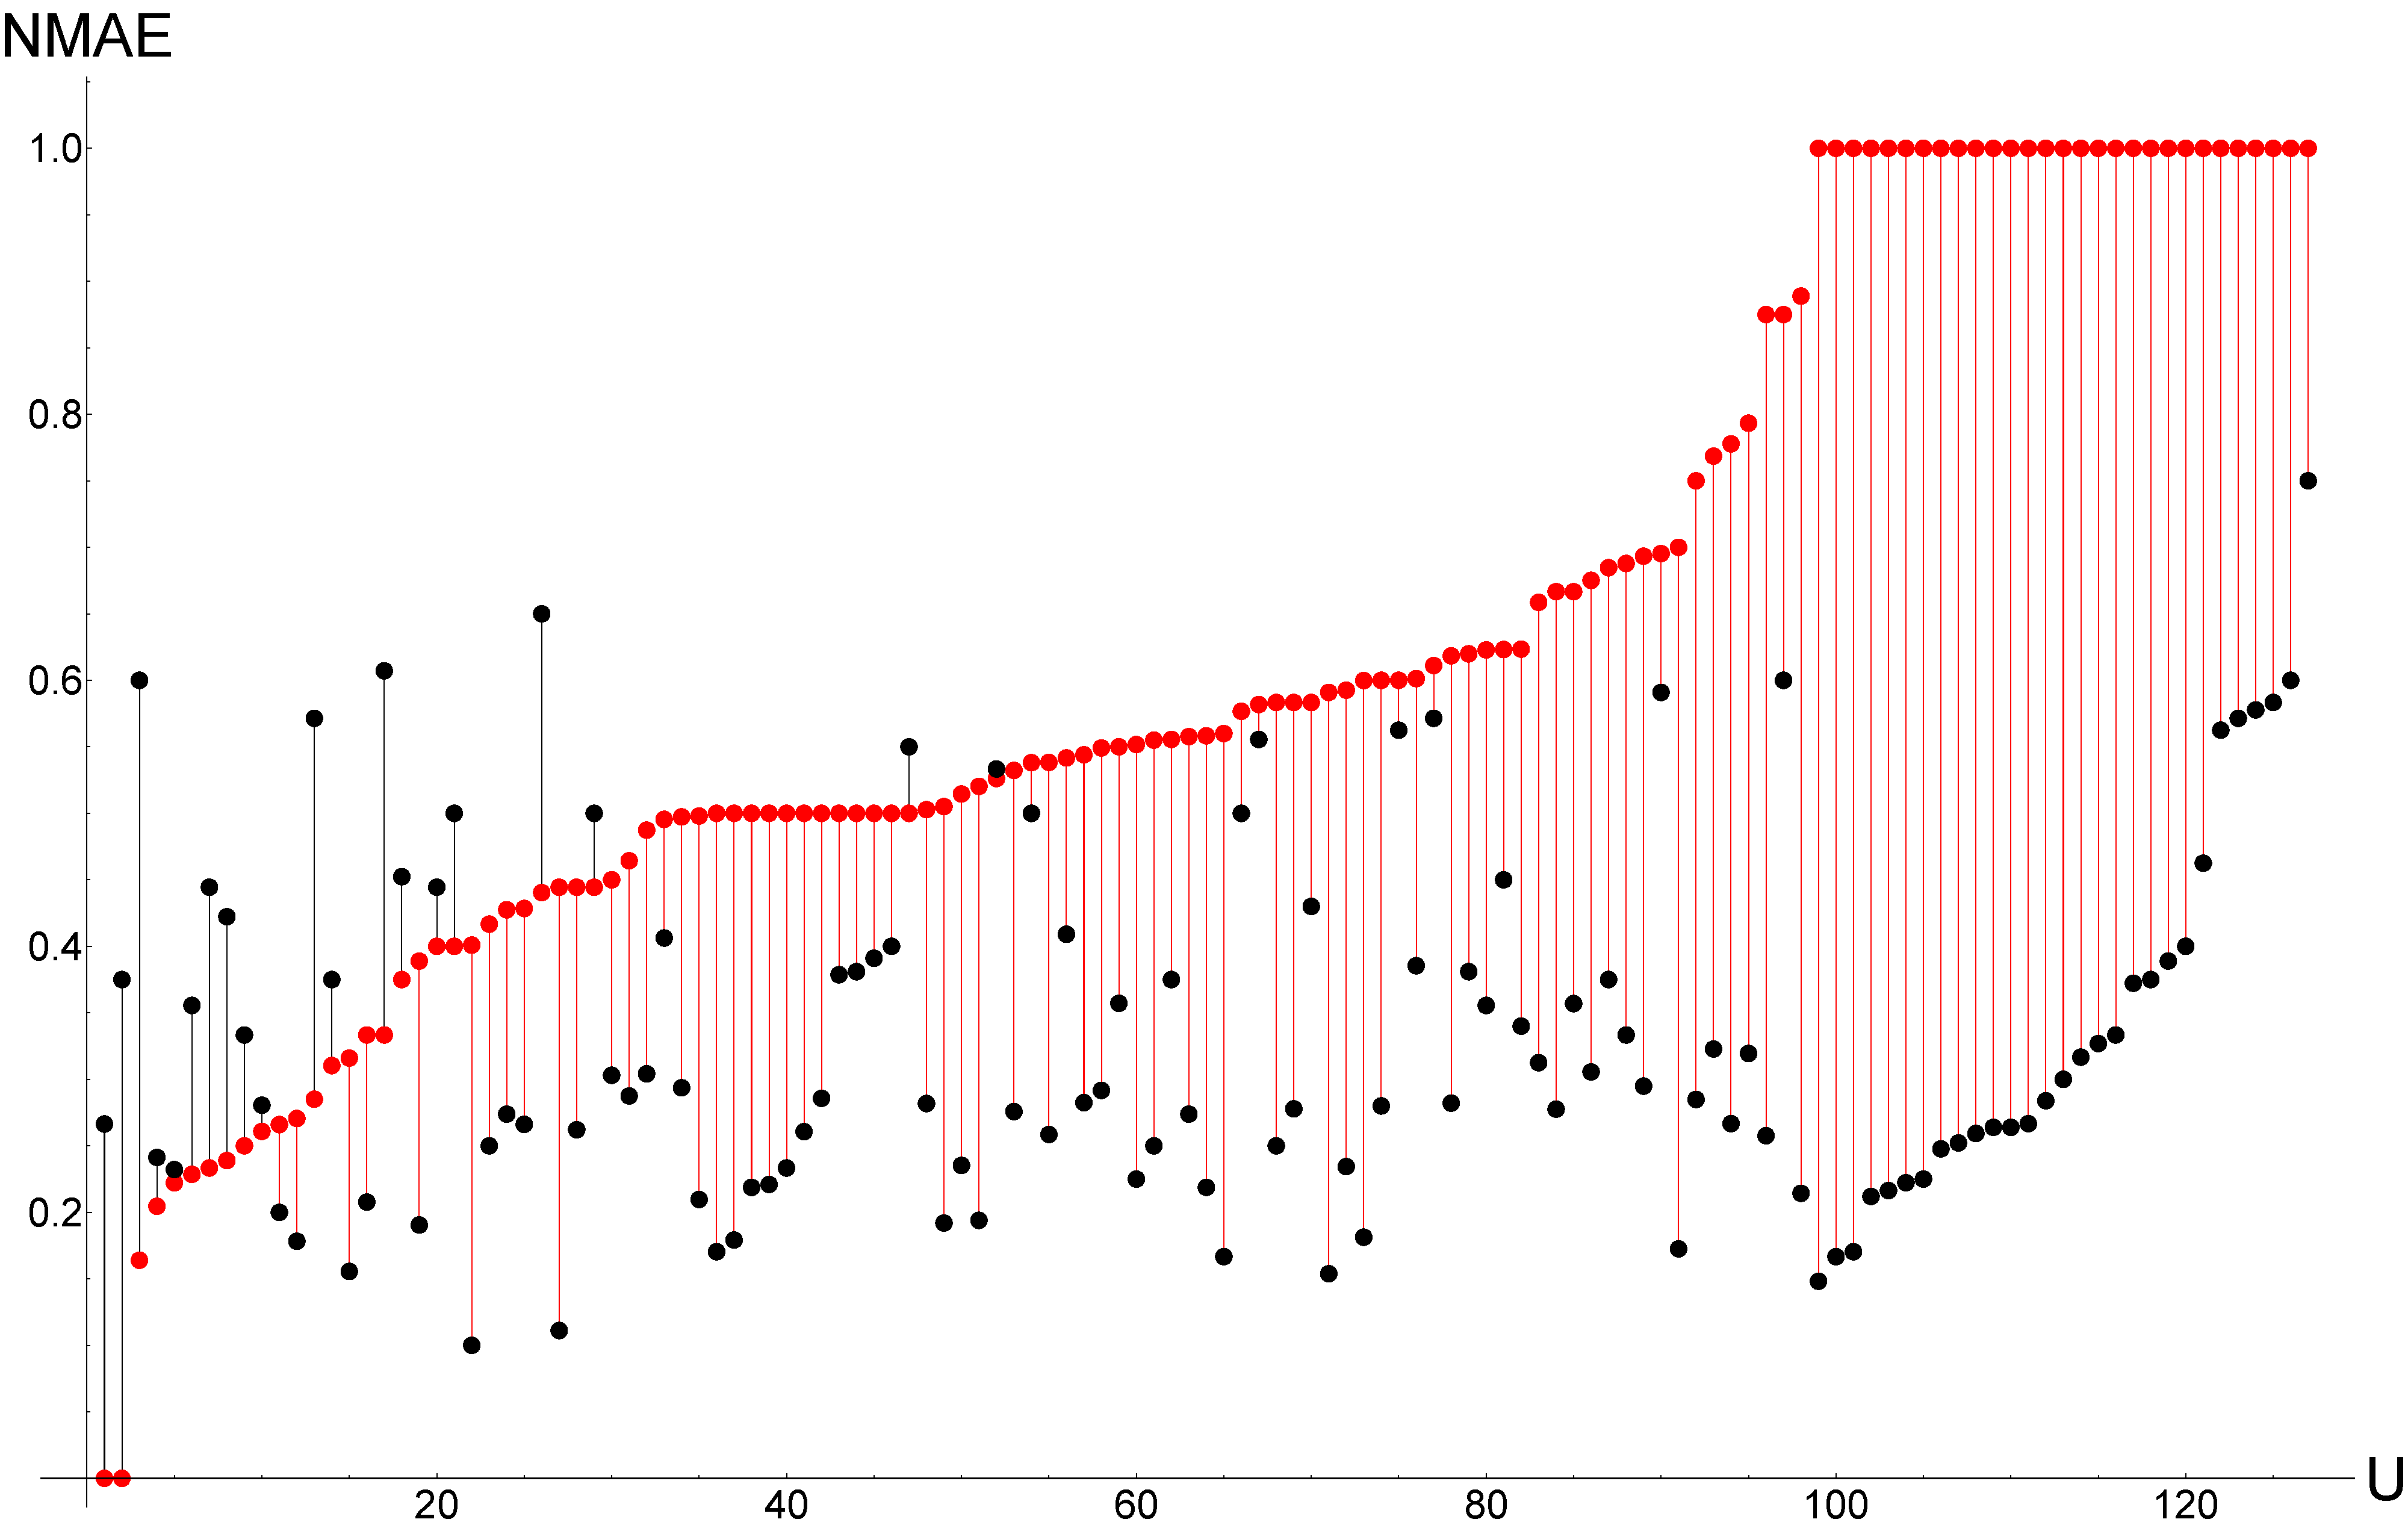
\includegraphics[width=7in,height=4in]{pics/results/ub_vs_fuzzy.pdf}
\end{center}
\end{figure}

\begin{table}[H]
	\caption{Средняя точность решений в СОМ и нечеткой модели при применении
	$\Pi_f$}
  \begin{center}
	\label{tbl:predfuz}
	\begin{tabular}{|c|c|}
	  \hline
		Модель/Правило вывода & Точность \\ \hline
		СОМ/$\Pi_{O}$&0,495\\ \hline
		Нечеткая/$\Pi_{f}$&0,334 \\ \hline
	\end{tabular}
  \end{center}
\end{table}


На Рис. \ref{pic:predpio_pif} приведены результаты решения
задачи $pred$ при применении $\Pi_C$ в СОМ и нечеткой модели.
Черным цветом обозначены результаты решения в нечеткой модели.
Видно, что в большинстве случаев нечеткая модель более эффективна
по критерию качества. В обратных ситуациях предпочтения пользователя
неоднородны, и $\delta_c$ для таких пользователей определена так, что
$|\rho(u, i) - \rh(u, i)| > \varepsilon_p$.

Практические результаты подтверждают вывод (\ref{trm:fuz-eff-extension}) о том,
что нечеткая модель является эффективным расширением АКМ по критерию качества.

